% This is "sig-alternate.tex" V2.1 April 2013
% This file should be compiled with V2.5 of "sig-alternate.cls" May 2012
%
% This example file demonstrates the use of the 'sig-alternate.cls'
% V2.5 LaTeX2e document class file. It is for those submitting
% articles to ACM Conference Proceedings WHO DO NOT WISH TO
% STRICTLY ADHERE TO THE SIGS (PUBS-BOARD-ENDORSED) STYLE.
% The 'sig-alternate.cls' file will produce a similar-looking,
% albeit, 'tighter' paper resulting in, invariably, fewer pages.
%
% ----------------------------------------------------------------------------------------------------------------
% This .tex file (and associated .cls V2.5) produces:
%       1) The Permission Statement
%       2) The Conference (location) Info information
%       3) The Copyright Line with ACM data
%       4) NO page numbers
%
% as against the acm_proc_article-sp.cls file which
% DOES NOT produce 1) thru' 3) above.
%
% Using 'sig-alternate.cls' you have control, however, from within
% the source .tex file, over both the CopyrightYear
% (defaulted to 200X) and the ACM Copyright Data
% (defaulted to X-XXXXX-XX-X/XX/XX).
% e.g.
% \CopyrightYear{2007} will cause 2007 to appear in the copyright line.
% \crdata{0-12345-67-8/90/12} will cause 0-12345-67-8/90/12 to appear in the copyright line.
%
% ---------------------------------------------------------------------------------------------------------------
% This .tex source is an example which *does* use
% the .bib file (from which the .bbl file % is produced).
% REMEMBER HOWEVER: After having produced the .bbl file,
% and prior to final submission, you *NEED* to 'insert'
% your .bbl file into your source .tex file so as to provide
% ONE 'self-contained' source file.
%
% ================= IF YOU HAVE QUESTIONS =======================
% Questions regarding the SIGS styles, SIGS policies and
% procedures, Conferences etc. should be sent to
% Adrienne Griscti (griscti@acm.org)
%
% Technical questions _only_ to
% Gerald Murray (murray@hq.acm.org)
% ===============================================================
%
% For tracking purposes - this is V2.0 - May 2012

\documentclass{sig-alternate-05-2015}

\usepackage{color}
\usepackage{booktabs}
\usepackage{tabularx}
\usepackage{graphicx}


\begin{document}

% Copyright
\setcopyright{acmcopyright}
%\setcopyright{acmlicensed}
%\setcopyright{rightsretained}
%\setcopyright{usgov}
%\setcopyright{usgovmixed}
%\setcopyright{cagov}
%\setcopyright{cagovmixed}


% DOI
\doi{10.475/123_4}

% ISBN
\isbn{123-4567-24-567/08/06}

%Conference
\conferenceinfo{PLDI '13}{June 16--19, 2013, Seattle, WA, USA}

\acmPrice{\$15.00}

%
% --- Author Metadata here ---
\conferenceinfo{WOODSTOCK}{'97 El Paso, Texas USA}
%\CopyrightYear{2007} % Allows default copyright year (20XX) to be over-ridden - IF NEED BE.
%\crdata{0-12345-67-8/90/01}  % Allows default copyright data (0-89791-88-6/97/05) to be over-ridden - IF NEED BE.
% --- End of Author Metadata ---

%\title{Alternate {\ttlit ACM} SIG Proceedings Paper in LaTeX
%Format\titlenote{(Produces the permission block, and
%copyright information). For use with
%SIG-ALTERNATE.CLS. Supported by ACM.}}
%\subtitle{[Extended Abstract]
%\titlenote{A full version of this paper is available as
%\textit{Author's Guide to Preparing ACM SIG Proceedings Using
%\LaTeX$2_\epsilon$\ and BibTeX} at
%\texttt{www.acm.org/eaddress.htm}}}
\title{I Can See Your Future! Analysing the Risk of Observable Callbacks in Android System }

%
% You need the command \numberofauthors to handle the 'placement
% and alignment' of the authors beneath the title.
%
% For aesthetic reasons, we recommend 'three authors at a time'
% i.e. three 'name/affiliation blocks' be placed beneath the title.
%
% NOTE: You are NOT restricted in how many 'rows' of
% "name/affiliations" may appear. We just ask that you restrict
% the number of 'columns' to three.
%
% Because of the available 'opening page real-estate'
% we ask you to refrain from putting more than six authors
% (two rows with three columns) beneath the article title.
% More than six makes the first-page appear very cluttered indeed.
%
% Use the \alignauthor commands to handle the names
% and affiliations for an 'aesthetic maximum' of six authors.
% Add names, affiliations, addresses for
% the seventh etc. author(s) as the argument for the
% \additionalauthors command.
% These 'additional authors' will be output/set for you
% without further effort on your part as the last section in
% the body of your article BEFORE References or any Appendices.

\numberofauthors{8} %  in this sample file, there are a *total*
% of EIGHT authors. SIX appear on the 'first-page' (for formatting
% reasons) and the remaining two appear in the \additionalauthors section.
%
\author{
% You can go ahead and credit any number of authors here,
% e.g. one 'row of three' or two rows (consisting of one row of three
% and a second row of one, two or three).
%
% The command \alignauthor (no curly braces needed) should
% precede each author name, affiliation/snail-mail address and
% e-mail address. Additionally, tag each line of
% affiliation/address with \affaddr, and tag the
% e-mail address with \email.
%
% 1st. author
\alignauthor
Chenkai Guo\\
       \affaddr{College of Computer and Control Engineering}\\
       \affaddr{Nankai University}\\
       \affaddr{Tianjin, China}\\
       \email{guochenkai88@gmail.com}
% 2nd. author
\alignauthor
Guangdong Bai\\
       \affaddr{School of Computing}\\
       \affaddr{National University of Singapore}\\
       \affaddr{Singapore}\\
       \email{baiguangdong@gmail.com}
% 3rd. author
\alignauthor 
Jinsong Dong\\
       \affaddr{School of Computing}\\
       \affaddr{National University of Singapore}\\
       \affaddr{Singapore}\\
       \email{dcsdjs@nus.edu.sg}
\and  % use '\and' if you need 'another row' of author names
% 4th. author
\alignauthor 
Jing Xu\\
       \affaddr{College of Computer and Control Engineering}\\
       \affaddr{Nankai University}\\
       \affaddr{Tianjin, China}\\
       \email{xujing@nankai.edu.cn}
% 5th. author
\alignauthor BalaBala\\
       \affaddr{NASA Ames Research Center}\\
       \affaddr{Moffett Field}\\
       \affaddr{California 94035}\\
       \email{fogartys@amesres.org}
% 6th. author
\alignauthor LabaLaba\\
       \affaddr{Palmer Research Laboratories}\\
       \affaddr{8600 Datapoint Drive}\\
       \affaddr{San Antonio, Texas 78229}\\
       \email{cpalmer@prl.com}
}

\maketitle
\begin{abstract}
The feature of event-driven acts as a key role that makes Android application differentiate from traditional PC software. For many of those events are hardly predicted and could not be observed by other applications, attackers are similarly impossible to engage corresponding attacks by finding the vulnerabilities of such an event-driven mechanism. However, of various kinds of events offered by either user or system, there are still events that can be received by more than one applications and further, could offer important basic resources to predict specific behaviours of targeted application.

PEC-threats(Public Events Callback)
In this paper, we perform a systematic study of such "public events" and their callback functions, and analyse potential security threats inside them. By exploiting the prediction capability of such callbacks, we demonstrate typical kinds of proof-of-concept attack examples, including spoofing, phishing and privilege escalation.
To evaluate the real influence of such threats, we implement a static analysis tool to detect a large scale of real world applications achieved from Google Play market. The detection result reveals such callback threats are pervasively existing in Android market applications. Since the threats involve in the fundamental design of the Android framework, it is very hard for ordinary developers and users to defense them. Given this challenge, we also proposed a migration strategy.

%The paper provides a sample of a \LaTeX\ document which conforms,
%somewhat loosely, to the formatting guidelines for
%ACM SIG Proceedings. It is an {\em alternate} style which produces
%a {\em tighter-looking} paper and was designed in response to
%concerns expressed, by authors, over page-budgets.
%It complements the document \textit{Author's (Alternate) Guide to
%Preparing ACM SIG Proceedings Using \LaTeX$2_\epsilon$\ and Bib\TeX}.
%This source file has been written with the intention of being
%compiled under \LaTeX$2_\epsilon$\ and BibTeX.
%
%The developers have tried to include every imaginable sort
%of ``bells and whistles", such as a subtitle, footnotes on
%title, subtitle and authors, as well as in the text, and
%every optional component (e.g. Acknowledgments, Additional
%Authors, Appendices), not to mention examples of
%equations, theorems, tables and figures.
%
%To make best use of this sample document, run it through \LaTeX\
%and BibTeX, and compare this source code with the printed
%output produced by the dvi file. A compiled PDF version
%is available on the web page to help you with the
%`look and feel'.

\end{abstract}


%
% The code below should be generated by the tool at
% http://dl.acm.org/ccs.cfm
% Please copy and paste the code instead of the example below. 
%
\begin{CCSXML}
<ccs2012>
 <concept>
  <concept_id>10010520.10010553.10010562</concept_id>
  <concept_desc>Computer systems organization~Embedded systems</concept_desc>
  <concept_significance>500</concept_significance>
 </concept>
 <concept>
  <concept_id>10010520.10010575.10010755</concept_id>
  <concept_desc>Computer systems organization~Redundancy</concept_desc>
  <concept_significance>300</concept_significance>
 </concept>
 <concept>
  <concept_id>10010520.10010553.10010554</concept_id>
  <concept_desc>Computer systems organization~Robotics</concept_desc>
  <concept_significance>100</concept_significance>
 </concept>
 <concept>
  <concept_id>10003033.10003083.10003095</concept_id>
  <concept_desc>Networks~Network reliability</concept_desc>
  <concept_significance>100</concept_significance>
 </concept>
</ccs2012>  
\end{CCSXML}

\ccsdesc[500]{Computer systems organization~Embedded systems}
\ccsdesc[300]{Computer systems organization~Redundancy}
\ccsdesc{Computer systems organization~Robotics}
\ccsdesc[100]{Networks~Network reliability}


%
% End generated code
%

%
%  Use this command to print the description
%
\printccsdesc

% We no longer use \terms command
%\terms{Theory}

\keywords{Android security; Information leaks; Permissions}

\section{Introduction}
Android platform has been already proven to be prevalent as a typical operating system installed in nowadays smartphone and tablet. Different from traditional PC program and software, applications within Android are event-driven and without a launching main function. That is to say, with different events, the program control flow would change correspondingly. Thus, call back mechanism that is used to response an event has played an important role in Android framework. 

Callback mechanism is originated from PC programs, which provides an asynchronous way for a specific class to invoke another's method when a certain event happens. In Android, callback functions reside everywhere of program structure in a typical app, especially in UI handling. For instance, after user click a button, a new activity would be popped up, presenting corresponding functionalities expected by user. In this case, a typical callback mechanism is used to response this specific user-click event. That is to say, the new activity would not be activated until user event happens. Besides, the events from system, other apps or life-cycle have similar callback responding mechanism.

On the other side, Android sandbox is known as an effect mechanism to protect apps from other one's attack. Sandbox restricts the resources to be offered for certain independent entities, leaving only very few ways for them to communicate with others. Actually, through the usage of conventional so-called side-channels, certain indirect inferring gradually evolves into a typical sort of attacks. In general, this sort of attacks threat a broad range of apps causing side-channels(such as process status) exist in system level. In other words, most of developed apps would be unable to avoid the influence brought by features from system level. Nevertheless, the impact appears limited for the deviation posed by sophisticated algorithms from current side-channel approaches. For instance, \cite{chen2014peeking}(UI state) treats several selected process statuses as side-channels, and utilizes them to infer a proper emergence time for the fake phishing Activity devised by attackers. However, the critical inference bases on a series of data collection and computations, leading to an inevitable derivation in term of device and targeted app itself. A typical example is that the typical Activity transition signal presence in \cite{chen2014peeking} is quite week and the shape is also changed in our reproducing experiment. Thus, using the same procedures as proposed in \cite{chen2014peeking} would hardly perform an ideal attack. The similar situation exists in other existing side-channel attacks aiming to Android apps as well \cite{zhou2013identity}\cite{jana2012memento}.

Compared to conventional side-channel attacks, we introduce a new type of potential threats called public event callback(PEC) threats, which leverage the weakness of public event callback mechanism within Android apps. Generally, callback functions expect a typical event to trigger their execution, and correspondingly the event is specified to sent to these callbacks. For example, the explicit intent specifies the single address(package name) of the target recipient and sends the intent out through a broadcast event. The broadcast only can be received by the specified single recipient. The entire broadcast process is properly protected by such single receiver mechanism. It is hard to obtain any data of such intent by other apps from the application level. However, not all the cases emerge so ideally. There still exists a large spectrum of public events that can trigger the execution of callbacks from different components and even different apps. We call this kind of callbacks PECs(public event callbacks).Examples includes system event, implicit intent, service running status, etc., which are insensitive on surface but offer attack materials for other apps with evil purpose. In particular, as the source of the expected event is possible to be exposed to public, the invoking time of a typical callback function could be inferred by other apps. As a result, the inferring result evolves to a variety of corresponding attacks directed against the display-sink, such as spoofing, phishing, privilege escalation, etc.    

However, the inferring process might not be as such simple as imaging. One challenge is that attackers have to fall into code level to gain necessary materials of victim apps overcoming the code confusion. Moreover, the attackers have to detect out at least one feasible inferring path across numerous control flow paths within targeted app. Such path has to contain a callback function that can be invoked by an exposed public event and a display-sink(e.g., startActivity or Toast.makeText) point with exposure features. The other challenge is that it should to be proven that there exists a determinable path from the start of such callback function to the display-sink, which involves more fine-grain analysis of program control flow. To achieve this goal, branch conditions and method invocation have to be properly handled to avoid the restriction of permission request and user-interaction.
Aiming at above challenges, we implement a statical analysis prototype tool CSDroid with 4k lines python codes to automatically conduct this inferring process to 2375** apps collected from Googly Play. Of all the targeted apps, we find 783** such sensitive paths within 354** targeted apps, including some popular apps like **. Moreover, it's surprising that 69\% **  of apps with service component suffer from such threats, which alerts us a high risk of such potential security threats within background components widely existing in generic apps.  

Given such an app with certain PEC weaknesses, an adversary attacker could devise a rich variety of attacks. Since such attacks are mainly based on the display-sink, the attack types are somehow similar with traditional UI attacks. However, as the display-sink should be reasonably inferred from the PEC, adversary app needs to concern more details about time-delay and program flow conditions. Besides that, traditional UI attacks mainly rely on activity display of victim app; display-sink contains more types of displays such as dialog and notification, which allow attackers to flexibly craft more attacks contents. To validate the feasibility of such PEC weaknesses exploitation, we explore and implement a set of proof-of-concept attacks based on such threats, including not only traditional phishing and spoofing to sensitive pages, but also newly dialog and notification exploitation for privilege escalation and other privacy steal. 

To migrate the impact of such PEC threats, we also discuss the defence strategy from two parts: Android system and developers. 

To summarize, the main contribution of this paper are:

1. We systematically study vulnerabilities of Android app lead by abuse of public event callbacks as well as discover various {\color{red}four} types of attack vectors leading to such PEC threats. 
 
2. By a set of corresponding proof-of-concept attacks, we validate the feasibility of such PEC exploitation and illustrate the severity of such threats. 

3. We introduce a tool implemented to automatically detect the PEC threats within targeted apps. By our study, a wide range of apps are affected by this kind of PEC attacks.

4. We provide a mitigation strategy to the PEC threats, under which a more security callback invoking mechanism can be established.

\section{Background}
In order to better understand the mechanism of this kind of attacks, firstly some relative background knowledge needs to be introduced.

\subsubsection{Events and Callbacks}
Events and callbacks are the ways that app interacts with Android system and users. Here, we define an \textit{event} as a situation that can trigger certain program logic to work. For instance, the explicit intent broadcast is such an event that can trigger a certain app receiving it and executing specific code after receiving.
Again, we define a \textit{public event} as situation that can trigger the programs logics from more than one app to work. Correspondingly, an implicit intent broadcast caters the definition of public event, which can be received by multiple apps. Apparently, the public event is the subset of the event.
Furthermore, we define a \textit{callback} as the code(e.g., function and program branch) that is executed after certain event(s) happen(s), and the execution is only related to such event(s). For example, an onClick method would only be executed after user clicks certain button. 

\subsubsection{Events in Android}
The trigger-events originated by different sources are equipped with different trigger features. For instance, a \textit{low-battery} event would happen only when the rest quantity of battery becomes as low as a pre-defined level, which is irrelevant to user's interaction. We categorize the events lied in Android that can lead to certain invocation of callback as three groups, namely \textit{life-cycle} event, \textit{user-driven} event, and \textit{system-driven} event.

\textbf{Life-cycle event} Android apps spontaneously arouse corresponding callback function according to the life-cycle step it resides. We call the event that can trigger life-cycle method to execute as life-cycle event. For instance, an Activity executes its \textit{onCreate} function when it is initially loaded, and executes the \textit{onPause} callback after it loses the screen focus. Life-cycle callbacks are somehow executed along with user's interactions and impacted by users. On surface, due to constraint of sandbox mechanism, the life-cycle phrases (Create,Pause,Destroy, etc.) of an given activity seem to be isolated from components belong to other apps. However, the event triggering certain life-cycle callbacks like onCreate and onDestroy enables other app to predict it in an indirect way. For example, the event that an activity is launching leads to the onCreate method in that activity executing. We conclude such life-cycle event that can expose the execution trace of certain app in Table 1.

\textbf{User-driven event} User-driven events interact with corresponding Android API in a direct way. User regularly are guided to perform diverse actions on screen, such as tapping, dropping up and down, click, double-click, etc., to operate a new app. Right after capturing an action from users, Android system would react following the  corresponding callback function that reflects the functionality and logic designed by developer. Generally, the user-driven event trigger the code execution of the one getting screen focus, which is hard capture by other apps. However, there still exists some user-driven events unrelated to the screen(e.g., shake action) acting as public events. 

\textbf{System event} System event normally come from the situation a given system status changes. If not specified, system event could be obtained by any app in theory so long as one is granted proper permissions. Generally, the permission granting could hardly attract user's attention for system event such as battery status is insensitive to user. To the end, system event provides an indirect entry for adversary app getting parts of the running process of other apps that implement system-driven callbacks interfaces. Table1 lists parts of system event instances.

\begin{table*}[t]
\centering
 \caption{\label{tab:test}Parts of events and callbacks in Android}
 \begin{tabularx}{\linewidth}{XXXXX} 
  \toprule
  Categories & Event & Callback & Permission & Public \\
  \midrule
  life-cycle & app starting & onCreate/onStart(launching activity); statical broadcast receiver & N/A & Y\\
             & activity losing focus & onPause & N/A & N\\
             & service starting & onCreate/onBind & N/A & Y\\
             
  user-driven & clicking button & onClick & N/A & N\\
              & shaking & onSensorChanged & N/A & Y\\
              
  system  & Intent.ACTION\_BATTERY\_LOW & onReceive & N/A & Y \\
          & Intent.ACTION\_BOOT\_COMPLETED & onReceive & RECEIVE\_BOOT\_COMPLETED & Y \\
  
  \bottomrule
 \end{tabularx}
\end{table*}

\subsubsection{Callback and Components}
Android platform is a kind of open source operating system established by Linux core. Developers could design and develop their own app product on Android in a flexible way, causing Android freely provides a variety of open source libraries and frameworks for developers. Of which, four types of components plays the key role in Android app's construction, namely \textit{Activity}, \textit{Service}, \textit{Broadcast Receiver} and \textit{Content Provider}. \textit{Activity} is designed as a graphical interface for interacting with users. Nevertheless, \textit{Service} is mainly used for handling complex computing job in background without a graphical user interface. \textit{Broadcast Receiver} provides a global listener that could trigger specific code logic when receive relative message. \textit{Content Provider} providers a universal interface for data storage and management, and for sharing data between different components. As a side-effect of user-driven mechanism, Android provides numerous of callback interfaces to be implemented by generic developers. Most of them rely on certain component, which we give greater details in follows.

\textbf{Callback in Activity} 
Most of callbacks in Activity are invoked by user-driven and life-cycle events, causing activity is mainly used for providing a visible graphic interfaces so as to interact with users. As aforementioned, upon the protection of sandbox, these callback statuses are hardly obtained by other apps only if the event triggered by user is irrelevant to screen focus. For instance, a shake action from users would lead to \textit{sensor} related events, which have no especial association with the screen. Besides, some system-driven callbacks are implemented in activity for catering the requirements of functionalities. 

\textbf{Callback in Service} 
Handling program logic and computing tasks in background, Service has no direct interaction with users, which is typically different from Activity. By this means, callbacks from service only come from life-cycle and system statuses. Yet, user's action without screen focus could be an exception, which we will discuss later.

Service life-cycle consists of five callback functions(onCreate, onStartCommand, onBind, onUnbind and onDestroy) but has a simpler life-cycle procedure compared with Activity. Being the same as Activity, these life-cycle callbacks are isolated from components of other apps so that has little utility value for attacker. 

Regularly, most of \textit{Services} are designed to wait for a typical signal and then invoke corresponding callback functions to push their computing result to an output interface, such as a \textit{dialog} or an \textit{Activity}. In general, the signal could be any type of event, invocation from other component or a program condition. If the trigger event belongs to system events, it can be easily obtained by component from other apps. This makes possible for attackers to perceive the execution process of a target app.

It is also possible to trigger a callback through a user-driven event in service, which is irrelevant to visible screen (e.g., shaking the phone to trigger SensorChanged event). Without specified receiver, this kind of events could be easily obtained by other apps either.   

\textbf{Callback in Broadcast Receiver} 
The \textit{Broadcast} has a wide spectrum of sources, from system or other components and can be delivered across all the installed apps through a common medium \textit{Intent}. Generally, callback functions in Broadcast Receiver only act as a channel that responses the coming Broadcast and then launches corresponding \textit{service} or \textit{activity} to handle it. However, once lacking of strong constraint, Broadcast Receiver could suffer from the threats of repeatedly receiving trash message from an adversary Broadcast sender. Similarly, it is also possible that a typical Broadcast is intercepted by a deliberately designed Receiver. Therefore, developers normally add some protection measures, such as setting the "export" property as false or using self-defined permission, to prevent from such attacks.

\textbf{Callback in Content Provider}
Content Provider acts as a channel for operating database in Android system, so callbacks in Content Provider appear quite trivial. Similar with Service, the Content Provider is designed as background component and its lifecycle callback onCreate() is mainly used to initialize the provider object. However, the provider is initiated when invoked by the operation from ContentResolver related to user-driven and program logic. Therefore, attackers are hard to leverage the process causing the launching time of a certain provider is hard to be captured by other apps. Besides, developers seldom set security related logics within onCreate() and other callbacks of Content Provider. Based on above consideration, we exclude the Content Provider in later PEC discussion.

\section{Exploiting Callbacks}
Android framework provides a variety of callback functions for developers conducting their apps a particular responding after a specific event happens. Yet, abusing these callbacks would incur undesirable consequence as well.
\subsection{Motivating Example}

\begin{figure*}[t]
\centering
\scalebox{1}[0.8]{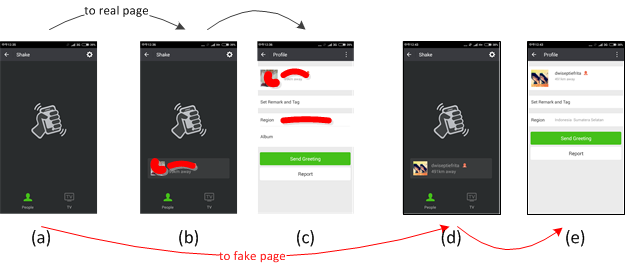
\includegraphics{pic1.png}}
\caption{\label{} Motivating example about the PEC threats. In (a), a user prepare to try the "Shake"; (b) shows a normal case that a real result popped up after shake; (c) presents the further information of such real page after user clicks the result; (d) shows the case that the shake action is perceived by an adversary app, which pop up a fake "result" page after it receives the shake action; (e) presents the further fake information crafted by attacker, which is used to induce user to convince it.}
\end{figure*}

We take the well-known app Wechat as a motivating example. Wechat is known as a popular IM(Instant Messenger) tool for users sharing information and connecting with each other. Of diverse functionalities it provides, "Shake" is rather welcomed, which enables users to randomly obtain an online chatting partner so long as slightly shaking the device several times.

Although harmony in surface, there exists potential crisis in the user shaking action which can be easily perceived by any other app through the {\color{red}SENSOR\_SERVICE}, a system service for managing inner device sensor. That is to say, only with the {\color{red}SystemSensorManager} object instantiation and the arrangement of shaking action size , an adversary app could clearly receive the same action event signal as Wechat. Further more, associating with the running status of Wechat through {\color{red}AMS(Activity Manager Service)}, adversary app could naturally make a judgement about the accurate time when the Wechat responding page would be popped up after user shaking. Although there exists an exception that user could shake the device in other page of "Wechat",the possibility of the exception's emergence is scarcely small in practice because user shakes device in such wide margin normally with intensive intention. {\color{red}Figure 1} shows how the "Shake" event is "stolen" by others. 

It seems that the PEC threats is easily ignored by developers and app markets. We see the callback time leakage severely because it offers a big change for attackers. A wily attacker could devise diverse attacks utilizing the PEC threats. For instants, attackers could deliberately construct a similar result page that links to a malicious third-party chatting tool, or even mimic a fake chatting page to pretend to chat with user for malicious purpose. We presents greater details about the attacks in section **.

\subsection{PEC Model} 

In order to clearly illustrate the callback threats, we view the threats process as a kind of callback state model. Each PEC within a installed app can be described as (S,D,E,C), where "S" denotes current state of app, which can be observed by other apps; "D" denotes the display-sink contained by the callback function; "E" denotes the event that invokes executing of the callback function; "C" denotes the proper control flow conditional values towards the "F".

\paragraph{Component-state}

(s belongs to S)The component-state refers to if the components of an app are running, which provides basic materials to PEC. Similar to the Event, the component-state here also needs to be exposed to other apps.

Before {\color{red}Android 5.0} emerging, the execution state of component like Activity and Service can be easily observed by the {\color{red}getRunningTasks API in ActivityManager object}. A more detailed observation needs to request the "GET\_TASK" permission, which could somehow attract the attention of most of normal users. However, Android starts to constraint the usage of such permission request and the usage of related API from recent {\color{red}Android 5.0+} for the security consideration. The getRunningTasks and even getRunningAppProcess(the API for get all the running process in the device) are now deprecated and only return developer's own application process. {\color{red}A substitute solution is to request new "PACKAGE\_USAGE\_STATS" permission, and to disable warning that permission is system level and will not be granted to third-party apps. Again, this approach needs extra permission request. } A decent solving method to get the foreground running app without any permission request is introduced in  \cite{getforeground} through reading the /proc file where Linux preserves all its process information. For all, obtaining the foreground app is entirely a completable task in common Android system version. 

Another good news is that the usage of  "getRunningServices" are still available in the newest version and need not request any extra permission. Thus, we can judge if a typical service is running through the "getRunningServices" API without any permission request. 

In addition, statically-registered BroadcastReceiver always in the receiving state when the app is running, so its component-state is also easy to ensure. On the other side, the component-state of dynamically-registered BroadcastReceiver follows the running state of its host component, e.g., activity and service, and the method where it is registered.


\paragraph{Display-sink}

(d belongs to D)Display Sink is based on the conception of leakage detection, which refers to a set of label functions that can expose data or information to outside. However, different from traditional conception, Display-sink here specifically refers to state output that could be perceived by users rather than information leakage, including UI page, dialog or notification, etc.

As to the Display-sink, only those output vectors which can be leveraged by attackers are considered. Most of which are related to UI activity, causing the UI is designed as the main channel to interact with users. Some of the UI vectors are mentioned in recent research\cite{bianchi2015app}(e.g., startActivity API, Toast message), yet we also collect some other UI related vectors, e.g., AlertDialog.Builder API, NotificationManager API. Generally, both of Dialog and Notification need response from users(e.g., click) and then engage corresponding reaction functionalities, which offers chance for attackers to interfere the users behaviours, which is insecure.

\textbf{Dialog}
Generally speaking, it goes against Android design and UI guidelines that directly launching a Dialog from Service or BroadcastReceiver. Therefore, if Dialog is roughly created from a Service or BroadcastReceiver, there would pop up an error report causing Dialog is implemented relying on a particular Activity. However, it is pretty work that setting a system alert Dialog with the "SYSTEM\_ALERT\_WINDOW" permission grant. This kind of Dialog has global feature that can be invoked by a Service or a system event rather than an Activity. 

\textbf{Toast}
In common case, the Toast is also constructed based on an existing Activity rather than Service or BroadcastReceiver. The reason of that is one of Toast.makeToast parameters refers to the main UI context the one belongs to. Therefore, directly popping up from Service or BroadcastReceiver would not work causing the UI context is erroneously referred. However, a common-used tool class "Handler" can be used to insert the self-defined thread message into the main thread queue, so that the main thread UI context can be obtained by the Toast. Therefore, Toast can be launched not only in Activity but also in Service and BroadcastReceiver.

\textbf{StartActivity}
The startActivity is known to be invoked by all the three components. However, some Activity is set self-defined permission to improve the security protection. For those low risk "protectionLevel", namely "normal" and "dangerous", we can still apply corresponding self-defined permission to access the target components. Nevertheless, for those high risk level, namely "signature" and "signatureOrSystem", currently there is no any effect way to access the target components by a third party app.

\textbf{Notification}
The Notification can be launched by all the three components as well. Compare to Dialog and Toast, Notification is more likely used in service for notify the task progress or updated information. 



Besides UI sink, some non-UI vectors are also contained, e.g., audio, vibrate related API, sendBroadcast, startService. Similar to UI related vectors, audio and vibrate related API also engage information output although as different information forms("voice and vibration"). The "sendBroadcast" and "startService" is able to lead new callbacks, which threatens the targeted app in a iterative way. Additionally, implicit intent loaded by "sendBroadcast" and "startService" also can be leveraged by attackers.

\paragraph{Event}

(e belongs to E) The event here refers to the public event since non-public one can hardly be exploited by other apps. As mentioned in section **, public events lie in all the three event categories(life-cycle, user-driven and system).



\paragraph{Control Flow}

(C)Control Flow is a collection of conditional values over the path from a typical State to a Display-sink. In theory, as for a callback threat vulnerable app, the "C" needs to guarantee an observable and feasible path that can reach the Display-sink. However, the "C" that strictly conforms above definition rarely emerges in real apps, so that we adopt a more flexible mechanism in practice which will be introduced in next section.  

Attackers need to find a feasible path from the State to the Display-sink within the given operable source code of a target app. For judging the existing of such path, we first collect the condition set of the paths to the Display-sink. Then a signal used to refer to if it is visible for each value, event and function emerging in the condition set is created. To describe more clearly, we denote the following concepts:

1. c: the condition value of each branch.

2. CS: the condition set collected from a program control flow path.

3. cv(a) : the condition value of variable a and a = variable | function | event

4. s(a): the signal value of variable a and a = variable | function | event, whose type is boolean.

s(a) represents if the variable a can be observed by components from other apps. s(a) = true represents yes, s(a) = false represents no.

5. CS = $\cap$ ( cv(a) \& s(a) ) = ($\cap$(c)) \& ( $\cap$ s(a))

Above equation means the value of condition set of a particular path consists of two parts, 1. the value of each variable; 2. the signal value of it.  A feasible path needs not only has a solvable condition set, but also observable for each variable. However, practically we normally use the second equation to compute the feasibility of a target path. First, computing out if it is feasible for each branch ; then , considering if it is able to be observed for each variable with the branch condition.

A traditional technique for above computation is symbolic execution. However, it needs unacceptable overhead in practice. {\color {red} To the end, we using an improved SMT approach to solve the constraint conditions.} Normally there should be feasible from source to sink in a target app, otherwise there exists a designation shortage with in the target app. Under this prerequisite, we only need to consider s(a), namely if all the variables are observable. 



\begin{figure}[t]
\centering
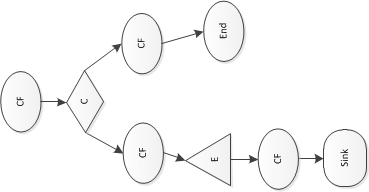
\includegraphics[width = 3.0in]{control-flow.png}
\caption{\label{}control-flow}
\end{figure}



\begin{figure}
\centering
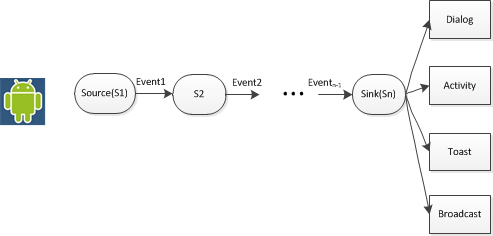
\includegraphics[width = 3.0in]{principle0.png}
\caption{\label{} principle0}
\end{figure}

\begin{figure}
\centering
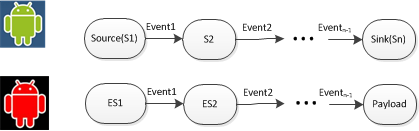
\includegraphics[width = 3.0in]{principle.png}
\caption{\label{}principle1}
\end{figure}



\begin{table*}[htbp]
\centering
 \caption{\label{tab:test} Typical vectors of PEC}
 %\begin{tabular}{lcll}
 \begin{tabularx}{\linewidth}{XXXX}

  \toprule
  State & Display-sink & Event & Control Flow \\
  \midrule
 1.Activity running state(Launching page) & 1.startActivity & 1.Broadcast from system: \{Intent.ACTION\_BATTERY\_LOW\} & 1.branch or cycle condition analysis \\
  2. Service running state &2. Toast message & 2.Implicit Intent\& pendingIntent & 2.method invocation analysis\\
     & 3.AlertDialog. Builder & 3.ServiceManager(need not permission grant): { sensorManager, memoryManager }\\
     & 4.sendBroadcast (intent)& 4.ServiceManager(need permission grant): { batteryManager }\\     
     & 5.AudioManager API & \\
     & 6.VibrateManager API & \\
     & 7.NotificationManager API & \\
     
  \bottomrule
 \end{tabularx}
\end{table*}



{\color{red}Table 2} lists the main vulnerability vectors with the callback threats. 

\section{Attack}

\subsection{Exploiting Condition}
\paragraph{App Description}
\paragraph{Timer}

\subsection{Threat Model}
In order to clearly illustrate the attack process, first the threat model need to be depicted.
Suppose that we have a victim app installed in a given device, and it contains corresponding callback threats vulnerabilities. Besides, suppose that we have an adversary app installed in the same device and start its service running on the background stealthily. The goal of our adversary app is to engage diverse attacks through the victim app. In theory, the adversary app need not apply any permission when it is installed. However, in practice, it needs to apply some  common-used permissions like "Internet" and insensitive permissions like "batter related permission" according to the attack type. The adversary needs to visually conceal its behaviours from users and also minimize its impact on the device performance. 

The adversary is supposed having the capability of using public available resources and analysing them on the fly. Again, it should stay aware of the running states of apps and some particular services. As introduced in "Callback State Model", this capability can be obtained by particular methods within ActivityManager class.

%\begin{table}
%\centering
%\caption{Frequency of Special Characters}
%\begin{tabular}{|c|c|l|} \hline
%Non-English or Math&Frequency&Comments\\ \hline
%\O & 1 in 1,000& For Swedish names\\ \hline
%$\pi$ & 1 in 5& Common in math\\ \hline
%\$ & 4 in 5 & Used in business\\ \hline
%$\Psi^2_1$ & 1 in 40,000& Unexplained usage\\
%\hline\end{tabular}
%\end{table}
%
%\begin{table}
%\centering
%\caption{Some Typical Commands}
%\begin{tabular}{|c|c|l|} \hline
%Command&A Number&Comments\\ \hline
%\texttt{{\char'134}alignauthor} & 100& Author alignment\\ \hline
%\texttt{{\char'134}numberofauthors}& 200& Author enumeration\\ \hline
%\texttt{{\char'134}table}& 300 & For tables\\ \hline
%\texttt{{\char'134}table*}& 400& For wider tables\\ \hline\end{tabular}
%\end{table}
% end the environment with {table*}, NOTE not {table}!
\begin{figure}
\centering
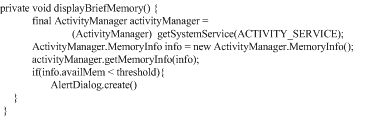
\includegraphics[width = 3.0in]{code1.png}
\caption{\label{}control-flow}
\end{figure}

\subsection{Attack Overview}

Following represents typical attacks forms that utilizes the PEC of victim app or PEC itself. According to the display-sink a PEC ends to, we representatively list several main types of attack examples, namely dialog \& toast privilege escalation, notification forgery, shaking-display spoofing and activity phishing. Meanwhile, we also introduce other possible attack types.
\subsection{Dialog \& Toast Privilege Escalation}
Dialog and Toast used to perform as the notice windows to notify users some intermediate results or alert information  after apps successfully receive events. Once the received events are open to public, an adversary app would be easy to predict the time when a dialog or toast really emerges as long as the targeted app lacks of complex condition constrains in its control flow of the key callbacks. A common case comes from the notice related to those system resources like battery, memory, voice, etc. Normally, these kinds of notices are sent by pre-installed or system manager apps. Also, users are with fully trust for these apps in security part because they are professional and have numerous of users. However, this trust acts as a big opportunity that can be exploited to achieve the attack goal in attacker's eyes.

For example, when the memory rests as low as a given level, some system manager apps(360 mobilesafe, Battery Doctor, etc.) would pop up corresponding dialog with alarm information("Dear user, your device has little memory available, clean the data residue to achieve more free memory?"), and if user clicks agree button, a new process launched by the manager app starts running. Then the user could be at ease at the memory trouble.

A typical implementation logic is represented as following:

The key point is the memory status(info.availMem) are public resources and can be obtained by any app installed in the device without any permission request. Moreover, the implementation control flow is designed so simple that 
the condition logic and variable "threshold" could be easily reconstructed in an adversary app. A experienced attacker could also obtain the these key logic and variables through reverse-engineering and binary analysis. As a result, the condition "info.availMem < threshold" as a public events makes the function "AlertDialog.create()" a PEC, and attackers are able to judge the creating time of the AlerDialog from its own reconstructed adversary app installed in the same device.

This time capture offers a rich variety of opportunities to engage attacks escaping user's notice, of which a typical one is privilege escalation. Figure * presents an attack procedure for an attacker getting the "Accessibility Service" grant by user. The Accessibility Service is a special functionality offered to help disabled people to get the component status and handle the device operations more conveniently. Since Android 4.0, it supports richer interfaces for developers implementing their Accessibility functionalities like listening user actions. Undoubtedly, this functionality is so powerful that it is impossible to be ignored by attackers. However, all the implementations have to be engaged under the prerequisite that user needs to open the Accessibility Service in setting options for a specific app. It seems infeasible for attackers to get the grant directly. After all, it performs very suspicious if such a setting window suddenly opens on the foreground against user's intention.

By exploiting the PEC of such a trusted app, all the attack procedure would become more reasonable. First, the adversary app opens a service on the background to monitor if the PEC service is running through the getRunningServices() offered by the ActivityManager. Fortunately, the invoking of getRunningServices() needs not any permission request and has not been constrained like the getRunningTasks()(mentioned in Section *) so far. Then, the adversary app construct the same logic as trusted app to wait for the time when the available memory size falls below the given threshold. Once it happens, the adversary app would predict the notice dialog will pop up in a few seconds. After that, it shows a toast tip to tell user the corresponding Accessibility Service have to be grant to complete the data clean task, and then opens the Accessibility Service setting page using "Setting.ACTION\_ACCESSIBILITY\_SETTINGS" intent like Figure *(b) did. In the setting page, an attack service with a confused name "360 Data Clean" makes user fool about this attack. At last, the adversary app gets the grant and could engage further attacks. 

 

Adversary apps also could utilize the callback logic within other apps. This is a more stealthy way. This kind of spoofing has various forms corresponding to the displayed windows of victim apps after a PEC happens.
1. Dialog. A victim system app is designed to give a data notice dialog when the month data rest below 150M. 

The display logic is located in the activity life-cycle function OnDestroy() which could be observed by adversary app outside. 

\subsection{Notification Forgery}
From perspective of practise, the Notification works for showing the received message, notifying the updated information and representing the progress of running tasks, which is somehow similar as Dialog or Toast. Different from the Dialog, it is not necessary to handle a Notification immediately. Again, a Notification would not disappear in seconds as the Toast does until user handles it. The user could handle it at any time they like, which gives attackers enough time to forge a fake one escaping user's attention. Here we introduce two common used situations. 

1. Push mechanism. Most of the market apps currently are based on CS(Client-Server) design, and the server needs to frequently push the updated data or content to the client in user's device. The client keeps running a service in the background receiving the update from server. Normally, this push-receive mechanism is implemented by specialized module with high-level security protection that makes it hard to get any status from the push process by other apps. However, causing the status of client service for receiving is publicly opened, attacker also could exploit it to fool the user in an indirect way. For example,the popular social app Google+ frequently uses the Notification to notify users to check its updated backup data, with two services PendingIntentCallbackService and DispatchingService running on the background. The status of these services could be easily observed by a third-party adversary app. Further more, the attacker has already analysed these services control flow off-line and found they connect to the Notification display. A fake Notification would be constructed using the same resources and framework as original Google+ did. The difference is the fake Notification are connected to a carefully constructed "Google login" page that needs user input their Google account. When the user open the Notification panel, there are several very similar Notifications listing there. If the user chooses the fake one and tries to log in the Google account, unfortunately, the username and password will be delivered to attacker.

2. Notice. Another important usage of the Notification is to notify users update status from a specific app or the device system. For instance, the QPtyhon(An app for python debugging on Android) would perform a log Notification when the OnDestroy() lifecycle function in the MainActivity happens. However, since the OnDestroy() is invoked when the MainActivity is destroyed, a third-party app could use the getRunningAppProcesses()(offered by ActivityManager) function to judge it. Thus, the OnDestroy() belongs to the PEC as well. Attackers could capture the time of such Notification emergence and even the time user triggers the Notification(when the targeted Notification is dismissed and corresponding app starts running.)by analysis from getActiveNotifications() offered by NotificationManager(after Android 4.3) 

Notification forgery. Figure * represents a notification forgery example. 

\subsection{Shaking-display Spoofing}
Shaking-display refers to the display(Dialog, Toast, Notification and Activity) led by a shaking action. A typical case comes from the motivation example we introduced in section 3.1**. The shaking action could be captured by the sensor in-set in the device. App developers normally use the sensorManager listener and its corresponding callbacks onSensorChanged() and onAccuracyChanged() to listen and handle the shaking action. Normally, the value of SensorEvent(parameter type of sensor callbacks) should be large enough to avoid the misrecognition of unexpected action without user's participating.

The shaking-display spoofing attack is based on the assumption that the shaking action always aims at the foreground activity. Since the shaking action always fits user's intention and in general cases, users only concern the foreground activity, the assumption is reasonable.

Consider the motivating example the Shake page pops up under two basic conditions. One is the WeChat is running on the foreground, and the other is shaking action event happens. As the assumption mentioned before, here we don't consider extreme situation that a device shaking happens accidentally in other page like the chatting page or setting page. Fortunately, both of the two conditions could be observed by public even without any of the permission request. 

Then let's consider another shaking-display spoofing example with the targeted app named "Digital Vulture". This app implements a novel usage that users could conveniently open the camera only needing slightly shaking the device several times. As analysis before, the handling function for responding the shaking event acts as a PEC. Therefore, an adversary app could capture when the camera is popped up by "Digital Vulture". At that time, a fake camera is launched by the adversary background service and covers on the face of original benign camera. The user is hard to distinguish the two camera surfaces and he/she is very likely to choose the fake one because it is on the foreground. Then adversary could stealthily deliver the picture to the web or store it in a secret location for other usage. The entire attack procedure is hard perceived by user. The only challenge that the adversary app has to overcome is to request the  "android.permission.CAMERA" permission. After all, the camera permission is not as sensitive as location or phone status for a user, so it is not hard for an attacker to get this non-sensitive permission.

\subsection{Activity Phishing}
Activity Phishing represents a more direct way to conduct the attack by the PEC. A traditional common used public event is the launching event of targeted app whose MainActivity contains private information input, e.g. login page and sign up page. An background adversary service keeps monitoring if the targeted app process begins running. Once the targeted page is launched, a forgery page with the same outlook would cover on the top surface and phish user's private data.

Here, we introduce a more complex PEC example related to implicit Intent. The implicit Intent is known as a bridge to connect another component without specifying a single receiver. Instead, it limits a range of receivers through making a operation statement including the intent data and the intended action. If an app sends an implicit Intent request and there are more than one apps fitting the Intent statement, the Android system would pop up a system dialog listing all the fitting apps. Then the user could choose one of them to handle the Intent data.

There exists a series of iterative PECs threats within the implicit Intent procedure. We still take the Wechat as an example. The Wechat providers a share feature that allows users to conveniently handle the received picture from other chatters. When the user long-presses the picture, a system dialog listing all the apps that can handle this picture pops up. Supposing that the user chooses the QQ, which means the user wants to send this picture to one of his/her QQ friends. As a result, the QQ login page pops up and the user could complete his/her intent after logging in the QQ.

As the analysis before, the running status of foreground app acts as a public event, so that the intent sender("com.tencent.mm" in this example) could be observed by an adversary app. Actually, the event that pops up the intent receiver QQ is also a public event and could be observed. Moreover, when the system dialog emerges for listing the receivers, the foreground process infers to the system dialog and the observable process name changes to "system:ui", which indicates the system dialog emerging is a public event as well. Therefore, there exists a PEC chain that contains sender app process, system dialog process and receiver process in sequence. By capturing the PEC chain, the adversary app could predict the emerging time of QQ login page and cover a phishing login page on the authentic one. Consequently, the adversary app could successfully bypass the unrelated pages(e.g., introduction page) and phish the login user name and password in an accurate way.

\subsection{Other Attacks}
The attacks discussed before are just typical attack types. There are still other attacks could be conducted using the PEC features. For instance, the Notification PEC also could be used to conduct the privilege escalation, only needing a reasonable spoofing page emerging when the user clicks the Notification icon. Again, shaking action could also be used to do phishing if the display is a sensitive login page. In addition, attackers even could try more flagrant attack forms, like ransoming user's critical data and ask for something they are interested for. To achieve this goal, attackers need to design a mal-block and pop it up once the targeted PEC happens. Actually, the attack is designed relying on the PEC type contained by victim app.

Another typical type of attacks follows a more direct and traditional way that utilizing PEC itself rather than a victim app. An adversary app could perform a customized response in terms of a targeted event. For example, adversary apps could be designed as a kind of spoofing pages, which would be popped up right after a particular event happens. The spoofing page content should be closely related to such event so that users have no doubt about it. Another example is to craft a fake phishing page for login that will pop up when the real app opens(the launching page is such a login page).

Table ** lists the possible associations of attack and the PEC.


\section{Detection and Evaluation}
This section we first analyse the detection details for the PEC and then provider an evaluation on a large scale of market apps.
\subsection{The PEC Detection}

To measure the PEC threats in real world apps, we designed a prototype tool CSDroid for detecting and analysing the PEC contained by market apps, which is implemented with 4k lines python code and based on the static analysing framework Androguard\cite{desnos2013androguard}. 

Our analysis includes four steps. 
First, we match the risk display with the source code of detected apps. We collect four types of risk display: Dialog, Toast, Notificaiton, and Activity, whose function features are listed in Table **. 

Then, the CSDroid would recognize the PEC vectors within the source code, including some of lifecycle callbacks of Activity \& Service, the callbacks of statically registered BroadcastReceiver and the callbacks defined as observable, e.g., onAccuracyChanged and onSensorChanged.

In the third step, the CSDroid backward traverses feasible method paths from risk displays to the PEC vectors. Generally, the callee methods invoked by the PECs are treated as observable, since these methods would be executed right after the execution of corresponding PECS according to control flow.

However, there are two challenges needed to overcome. 
First, it is inevitable that some apps contain iterative such method traces. For example, a background service is waiting for a public event and then would launch a new activity. Similarly, in the new activity, the execution of onCreate() lead to a notice dialog poping up. This case exists an iterative method path that the PEC of service first transmits to the activity, and then the activity PEC transmits to the dialog. We use redirecting PEC to handle this iterative cases. Considering the joints of an iterative path are always code-block for activity launching(code-block of method startActivity), such as the case introduced above, we model four types of intents used to launch a new activity and flag the target activity name within the intent. After that, in the rest of the method traces, if there is a PEC activity name being the same as the flagged one, the CSDroid associates the two methods, and as a result, the two method traces(one is ended by the startActivity referring to the flagged activity; the other is started by the flagged activity) are integrated as an iterative one.

The second challenge is that not all the extracted PEC method traces are observable for other apps.
On the one hand, the adversary app is supposed to be installed without sensitive permission grant. In this way, the PEC path with a system API that needs permission grant is hard to be observed to an adversary app. On the other hand, features involving private resources of the targeted app are also forbidden to observe. For instance, the statical-registered BroadcastReceiver is regarded as a PEC. Yet, an explicit intent that specifies the single receiver's name, received by the objective BroadcastReceiver, could not be observed by other app at all.

The CSDroid analysing such violation situations in a fine-grain way. To solve the permission API problem, considering that the key impact of such a permission grant API is able to confuse the direction of control flow, CSDroid focuses on handling the branch conditions containing such API, with three steps. First, to a method node N whose predecessor method node is denoted as M, CSDroid tells accurate position P in the body of M where N is invoked. Then, from position P, CSDroid conduct a backward traversing to detect whether P potentially depends on a branch condition(we denote such branch condition as B if it exists). If such branch condition exists, CSDroid would recognize whether it depends on a permission grant API through dependency flow analysis. Our permission grant API database comes from the project of PScout\cite{au2012pscout} which offers a complete mapping list for Android system permission and API. If a permission dependency branch condition is recognized, the CSDroid would remove it from existing method traces.

Compared to the permission API problem, CSDroid just easily build a whitelist to exclude such method traces with any of private resources feature.



\# handling of inner class  

\subsection{Market-scale Study}
Our analysis is targeted on 2,723 real-world apps crawled by Google Play in 2016, covering all the 27 categories. The final detection results are listed in Table **.


\subsection{Vulnerability Discuss}

\section{Migration Strategy}
The conditions that enable the attacks successful come from three parts. First, Android system allows the existence of such PECs (metioned in section **). Second, app developers ignore the PEC problem during their developing process. Third, users have little awareness about such PEC attacks. The violation of any condition would make the attacks fail. Therefore, to migration work should start with above three parts.
 
System Level. The observation to activity status is known to be prevented from other task stacks in Android 5 and newer versions. It brings substantial benefits for protection of app status from being stolen during runtime. However, the status of components like service, launching activity and broadcastreceiver still can be observed or predicted. Besides that, it is free to access some insensitive-in-surface system resources such as the sensor data. Again, system events can be received by more than one entities at the same time. All above system design makes the PEC attack possible. Therefore,   Android system could conduct effective improvement aiming to above features. Compared with changing the event receiving mechanism which involves entire design of Android framework, adding reasonable access to obtain particular resources or observe specific components appears more feasible. However, it is a trade-off between security threats and existing functionalities after all. We expect Android has a concrete improvement for this concern in later versions.

Application Level. From our market survey of the PEC threats, numbers of real-world apps leave the possibility of being attacked by malware through such threats. One clear way to address such problem is to provide a reasonable guideline for developers to avoid this threats during their developing process. Some safety developing habits would be intensively suggested, such as don't set the log-in page in the launching activity, don't link a service to a sensitive activity or dialog, don't pop up a sensitive window right after a system event happens, etc. The developers should also clearly consider related factors based on such tradeoff between security and functionality before developing. However, it seems impossible for a vendor to constrain it's app products as such suggests, which appears overstrict for developers since only a small part of such "unqualified products" suffer from real attacks in practice. To address this challenge, users are expected to be presented a notification tip asking them to whether approve or not when a new display is built after a certain public event. Such notification guides users to be aware of the PEC threats, which is what we strive to in the next stage.

 


\section{Related Work}

Android Event-driven Analysis
Based on event-driven mechanism, Android application adopts a much flexible execution way, which makes it hard to be directly analysed like the one on conventional personal computer. Researchers has done much efforts on tackling this challenge. \cite{yang2015static} fundamentally proposes a program representation built by context-sensitive static analysis of callback methods to model the app's GUI. \cite{kim2014fepma} provides an event-driven analysis manner to measure the power dissipation.  \cite{chen2013contextual} centres around so-called Permission Event Graph built with static analysis and uses model checking to illegal interaction between an application and the Android event system. Again, \cite{jensen2013automated} handle event-driven analysis to reach challenging source code for application testing. \cite{machiry2013dynodroid} presents Dynodroid to monitor the reaction of an app upon each event either from system or user. \cite{hsiao2014race}presents a race detection tool named CAFA for event-driven mobile systems. Although prior works present different insights of event-driven analysis in Android system, there are few efforts concerning the security impact raised by public event abuse. Our work fills this gap via systematic study of Android system design and statical analysis for a large scale of real-world apps.

Android Defects Exploitation
The exploration and exploitation of weaknesses within either Android system or apps are intensively focused by current related researchers. The study of memory side-channel analysis and exploitation\cite{zhou2013identity, chen2014peeking, jana2012memento}uncovers an indirect attack way aiming to the weak architecture of Android public data exposure.
Several recent researches focus on the vulnerabilities raised by Android advertising libraries\cite{soteris2016free}\cite{sooel2016mob_ads}. Besides that, \cite{zhang2016life} proposes data residue problem during app uninstallation. As a direct interaction channel with users, the Android UI also suffers from severity security threats, which is carefully discussed in \cite{ren2015towards}\cite{bianchi2015app}\cite{akhawe2014clickjacking}\cite{luo2012touchjacking}\cite{huang2012clickjacking}\cite{roesner2013securing}\cite{lin2014screenmilker}. 
Again,in the work of \cite{mylonas2013smartphone}\cite{xu2012taplogger}\cite{miluzzo2012tapprints}, the sensor data could also be regarded as a sort of attack resources predicting some isolated private information including user input,fingerprints. In addtion, \cite{armando2012dos} introduces a denial-of-service attack approach utilizing the AMS design defect. \cite{xing2014upgrading} and \cite{bugiel2012towards} present detailed studies about privilege escalation for malware through defects of Android os.  As to Android permission mechanism, \cite{felt2011android}\cite{au2012pscout}\cite{zhang2013vetting}\cite{fang2014permission} reveal security threats arised by the abuse of permission requests and propose corresponding migration strategy.
In contrast to existing work, this paper represents the impact of public event defect of Android that affects a much wider range of system components and services. The attacks relying on such public event callbacks are firstly studied systematically.

Android Vulnerability Detection
As a critical security concerning on Android system, privacy data leakage incurs widely related research efforts. 
Of all the detection works, dynamic taint tracking \cite{enck2014taintdroid}\cite{klieber2014android}\cite{rastogi2013appsplayground}\cite{poeplau2014execute} receives much eyesights for its sound accuracy.
Another important complement for dynamic approach relies on static analysis\cite{lu2012chex}\cite{arzt2014flowdroid}\cite{gordon2015DroidSafe}, which can effectively reduce the false negative rate. Further works concern the impacts of ICC(inter-component communication) mechanism\cite{cao2015edgeminer}\cite{octeau2013epicc}\cite{li2015iccta}. In addition,
\cite{cox2014spandex} measures implicit leak of user password using symbolic execution. Our work is devoted to uncover the public event threats within real market app, which can be easily exploited by attackers to build a wide spectrum of new malwares. 
















\section{Conclusions}

%of the reference to the \LaTeX\ book, the citations in
%this paper are to articles which have nothing to
%do with the present subject and are used as
%examples only.
%\end{document}  % This is where a 'short' article might terminate

%ACKNOWLEDGMENTS are optional
\section{Acknowledgments}
%This section is optional; it is a location for you
%to acknowledge grants, funding, editing assistance and
%what have you.  In the present case, for example, the
%authors would like to thank Gerald Murray of ACM for
%his help in codifying this \textit{Author's Guide}
%and the \textbf{.cls} and \textbf{.tex} files that it describes.

%
% The following two commands are all you need in the
% initial runs of your .tex file to
% produce the bibliography for the citations in your paper.

\bibliographystyle{abbrv}

\bibliography{sigproc}
  % sigproc.bib is the name of the Bibliography in this case
% You must have a proper ".bib" file
%  and remember to run:
% latex bibtex latex latex
% to resolve all references
%
% ACM needs 'a single self-contained file'!
%
%APPENDICES are optional
%\balancecolumns
\appendix
%Appendix A
\section{Headings in Appendices}
%The rules about hierarchical headings discussed above for
%the body of the article are different in the appendices.
%In the \textbf{appendix} environment, the command
%\textbf{section} is used to
%indicate the start of each Appendix, with alphabetic order
%designation (i.e. the first is A, the second B, etc.) and
%a title (if you include one).  So, if you need
%hierarchical structure
%\textit{within} an Appendix, start with \textbf{subsection} as the
%highest level. Here is an outline of the body of this
%document in Appendix-appropriate form:
%\subsection{Introduction}
%\subsection{The Body of the Paper}
%\subsubsection{Type Changes and  Special Characters}
%\subsubsection{Math Equations}
%\paragraph{Inline (In-text) Equations}
%\paragraph{Display Equations}
%\subsubsection{Citations}
%\subsubsection{Tables}
%\subsubsection{Figures}
%\subsubsection{Theorem-like Constructs}
%\subsubsection*{A Caveat for the \TeX\ Expert}
%\subsection{Conclusions}
%\subsection{Acknowledgments}
%\subsection{Additional Authors}
%This section is inserted by \LaTeX; you do not insert it.
%You just add the names and information in the
%\texttt{{\char'134}additionalauthors} command at the start
%of the document.
\subsection{References}
%Generated by bibtex from your ~.bib file.  Run latex,
%then bibtex, then latex twice (to resolve references)
%to create the ~.bbl file.  Insert that ~.bbl file into
%the .tex source file and comment out
%the command \texttt{{\char'134}thebibliography}.
% This next section command marks the start of
% Appendix B, and does not continue the present hierarchy
\section{More Help for the Hardy}
%The sig-alternate.cls file itself is chock-full of succinct
%and helpful comments.  If you consider yourself a moderately
%experienced to expert user of \LaTeX, you may find reading
%it useful but please remember not to change it.
%\balancecolumns % GM June 2007
% That's all folks!

\end{document}
